\documentclass[a4paper,10pt,ngerman]{scrartcl}
\usepackage{babel}
\usepackage[utf8x]{inputenc}
\usepackage[a4paper,margin=2.5cm,footskip=0.5cm]{geometry}

% Die nächsten vier Felder bitte anpassen:
\newcommand{\Aufgabe}{Aufgabe 1: Arukone}               % Aufgabennummer und Aufgabennamen angeben
\newcommand{\TeamId}{00054}                             % Team-ID aus dem PMS angeben
\newcommand{\TeamName}{K7Bots}                          % Team-Namen angeben
\newcommand{\Namen}{Konstantin Kuntzsch}                % Namen der Bearbeiter/-innen dieser Aufgabe angeben
 
% Kopf- und Fußzeilen
\usepackage{scrlayer-scrpage, lastpage}
\setkomafont{pageheadfoot}{\large\textrm}
\lohead{\Aufgabe}
\rohead{Team-ID: \TeamId}
\cfoot*{\thepage{}/\pageref{LastPage}}

% Position des Titels
\usepackage{titling}
\setlength{\droptitle}{-1.0cm}% Für mathematische Befehle und Symbole
\usepackage{amsmath}
\usepackage{amssymb}

% Für Bilder
\usepackage{graphicx}

% Für Algorithmen
\usepackage{algpseudocode}

% Für Quelltext
\usepackage{listings}
\usepackage{color}
\definecolor{mygreen}{rgb}{0,0.6,0}
\definecolor{mygray}{rgb}{0.5,0.5,0.5}
\definecolor{mymauve}{rgb}{0.58,0,0.82}
\lstset{
  keywordstyle=\color{blue},commentstyle=\color{mygreen},
  stringstyle=\color{mymauve},rulecolor=\color{black},
  basicstyle=\footnotesize\ttfamily,numberstyle=\tiny\color{mygray},
  captionpos=b, % sets the caption-position to bottom
  keepspaces=true, % keeps spaces in text
  numbers=left, numbersep=5pt, showspaces=false,showstringspaces=true,
  showtabs=false, stepnumber=2, tabsize=2, title=\lstname
  }
\lstdefinelanguage{JavaScript}{ % JavaScript ist als einzige Sprache noch nicht vordefiniert
  keywords={break, case, catch, continue, debugger, default, delete, do, else, finally, for, function, if, in, instanceof, new, return, switch, this, throw, try, typeof, var, void, while, with},
  morecomment=[l]{//},
  morecomment=[s]{/*}{*/},
  morestring=[b]',
  morestring=[b]",
  sensitive=true
}

% Diese beiden Pakete müssen zuletzt geladen werden
%\usepackage{hyperref} % Anklickbare Links im Dokument
\usepackage{cleveref}

% Daten für die Titelseite
\title{\textbf{\Huge\Aufgabe}}
\author{\LARGE Team-ID: \LARGE \TeamId \\\\
	    \LARGE Team-Name: \LARGE \TeamName \\\\
	    \LARGE Bearbeiter/-innen dieser Aufgabe: \\ 
	    \LARGE \Namen\\\\}
\date{\LARGE\today}

\begin{document}

\maketitle
\tableofcontents

\vspace{0.5cm}

\section{Lösungsidee}
\begin{flushleft}
    Die Lösungsidee besteht darin, zuerst eine spezielle Struktur von Zahlen in eine Ecke des Gitters zu platzieren. Der 2. Teil des Gitters wird dann so mit Zahlen gefüllt, dass dieser Teil für sich gesehen immer lösbar ist.
    \linebreak
    \linebreak
    Der 1. Teil besteht dabei aus einer Struktur, die, wenn sie auf die richtige Art in einer Ecke platziert wird, zwar lösbar ist, an der das Lösungsprogramm aber scheitert.
    \linebreak
    \linebreak
    Die Struktur, inklusive der theoretisch möglichen Lösung, ist in \cref{abb:bild1} dargestellt.
    \linebreak
    \linebreak
    Der Lösungsalgorithmus funktioniert, indem er das Paar gleicher Zahlen heraussucht, bei dem der kürzestmögliche Weg zwischen den beiden Zahlen unter allen Paaren am kleinsten ist. Haben zwei Paare einen gleich langen kürzesten Weg, wird das Paar mit der kleineres Zahl bevorzugt. Die Zahlen des so ausgewählten Paares werden nun auf dem kürzestmöglichen Weg miteinander verbunden. Dieser Vorgang wird solange wiederholt, bis kein Paar übrig ist.
    \linebreak
    \linebreak
    Im Fall der \glqq{Fallen}\grqq-Struktur bedeutet das, dass zuerst die beiden Zahlen 1 miteinander verbunden werden, da diese, wie die Zahlen 2, den Abstand 4 haben, die 1er jedoch aufgrund der kleineren Zahl priorisiert werden. Dadurch wird der, aufgrund der Platzierung in der Ecke, einzige Weg, die 2en zu verbinden, blockiert, sodass das Rätsel unlösbar wird, wie in \cref{abb:bild2} sichtbar ist.
    \linebreak
    \linebreak
    Dadurch wird ein Rätsel erstellt, welches zwar lösbar ist, jedoch durch das Lösungsprogramm nicht gelöst werden kann, die Bedingungen der Aufgabenstellung werden also erfüllt.
    \linebreak
    \linebreak
    Um mehr Variationsmöglichkeiten zu erzeugen, werden 1. die \glqq{Fallen}\grqq-Struktur gespiegelt, gedrekt und dementsprechend in einer anderen Ecke platziert und 2. die anderen Paare zufällig angeordnet.
\end{flushleft}

\begin{figure}
    \begin{center}
        \includegraphics[width=0.3\textwidth]{images/falle_lösung.png}
        \caption{Die \glqq{Fallen}\grqq-Struktur und die mögliche Lösung}
        \label{abb:bild1}
    \end{center}
\end{figure}

\begin{figure}
    \begin{center}
        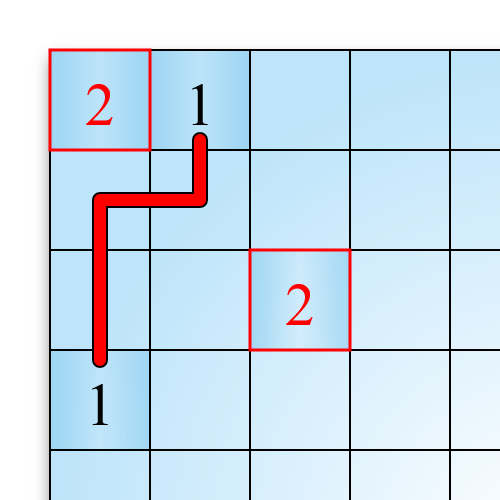
\includegraphics[width=0.3\textwidth]{images/falle_versuch.png}
        \caption{Die \glqq{Fallen}\grqq-Struktur und der Versuch des Lösungsprogramms}
        \label{abb:bild2}
    \end{center}
\end{figure}

\section{Umsetzung}
Die Umsetzung dieser Aufgabe erfolgt in Python, einer Programmiersprache, die für ihre Einfachheit und Lesbarkeit bekannt ist.
Der Code ist in folgende Bereiche unterteilt:

\subsection{Datenstrukturen}
\subsubsection*{SchemaPunkt}
Die SchemaPunkt-Struktur repräsentiert einen Eintrag in einem Schema, bestehend aus X- und Y-Koordinate sowie der entsprechenden Zahl am angegebenen Gitterfeld.

\subsubsection*{Schema}
Die Schema-Struktur repräsentiert ein Schema wie die \glqq{Fallen}\grqq-Struktur, bestehend aus einer Liste von SchemaPunkten.

\subsubsection*{Arukone}
Die Arukone-Struktur repräsentiert ein fertiggestelltes Arukone-Rätsel, bestehend aus einer Liste von Zeilen, die jeweils als eine Liste von Zahlen dargestellt werden.

\subsection{Eigentlicher Algorithmus}
Die Funktion \texttt{erstelle\_arukone()} ist dafür zuständig, ein Arukone-Rätsel der angegebenen Größe zu erstellen.
Dabei wird die Funktion \texttt{erstelle\_falle()} aufgerufen, welche eine zufällige Fallenstruktur erzeugt.

\subsubsection{Erstellen der Fallenstruktur}
\begin{flushleft}
      Das Erstellen der Fallenstruktur erfolgt, indem zuerst eine lokale Variable \texttt{schema} mit einer Ursprungsvariation der Fallen-Struktur initialisiert wird.
      \linebreak
      \linebreak
      Außerdem werden die Variablen \texttt{ist\_oben} (mit dem Wert \texttt{True}) und \texttt{ist\_links} (mit dem Wert \texttt{False}) initialisiert, welche angeben, in welcher Ecke die Struktur platziert werden soll.
      \linebreak
      \linebreak
      Im Folgenden werden diese drei Variablen dann zufällig verändert, um zufällig eine der acht möglichen Variationen der Struktur zu erzeugen.
      Dabei wird in drei voneinander unabhängigen Schritten jeweils zufälllig entschieden, ob eine bestimmte Transformation auf das Schema und die Variablen angewendet wird, oder nicht.
      \linebreak
      \linebreak
      Diese 3 Schritte sind:
      \begin{enumerate}
            \item Spiegeln des Schemas durch Vertauschen der X- und Y-Koordinaten aller SchemaPunkte
            \item Drehen des Schemas um 180° durch getrenntes Spiegeln der X- und Y-Koordinaten aller SchemaPunkte
            \item Drehen des Schemas um 90° durch Vertauschen der X- und Y-Koordinaten aller SchemaPunkte und anschließendes Spiegeln der X-Koordinaten
      \end{enumerate}
      Durch diese Transformationen können sowohl alle vier möglichen Drehungen (0°, 90°, 180°, 270°) als auch gespiegelte bzw. nicht gespiegelte Variationen erzeugt werden.
      \linebreak
      \linebreak
      Als letzter Schritt berechnet die Funktion \texttt{erstelle\_falle()} ausgehend von \texttt{ist\_oben} und \texttt{ist\_links}, sowie der als Parameter an die Funktion übergebenen Größe des Rätsels, die endgültige Position der Falle im Rätsel und addiert die entsprechenden X- und Y-Werte zu allen SchemaPunkten.
      \linebreak
      \linebreak
      Die Funktion gibt das Schema, \texttt{ist\_oben}, \texttt{ist\_links} und die Breite bzw. Höhe des Schemas als ein \texttt{tuple} zurück.
\end{flushleft}

\subsubsection{Vervollständigen des Arukone-Rätsels}
\begin{flushleft}
      Die Funktion \texttt{erstelle\_arukone()} erstellt zuerst eine Liste bestehend aus $n$ Listen, welche wiederum $n$ mal die Zahl $0$ enthalten. Diese Liste stellt die Kästchen und Ziffern im Rätsel dar.
      Außerdem wird die Anzahl der Zahlenpaare des zu erstellenden Rätsels als $n / 2$, gerundet auf die nächstgrößere Ganzzahl, berechnet.
      \linebreak
      \linebreak
      Daraufhin wird durch \texttt{erstelle\_falle()} eine zufällige Fallenstruktur erzeugt und in die erstellte Struktur eingefügt.
      \linebreak
      \linebreak
      Zum Schluss müssen genug weitere Zahlenpaare eingefügt werden, sodass insgesamt mindestens $n/2$ Zahlenpaare im Rätsel vorhanden sind.
      Dafür wird zuerst $n$ durch $2$ dividiert und das Ergebnis aufgerundet, um die Anzahl der Zahlenpaare zu erhalten.
      \linebreak
      \linebreak
      Daraufhin wird mithilfe einer Zählschleife von $3$ bis zu (inklusive) der Anzahl der Paare gezählt (Start bei $3$, da die Fallenstruktur bereits zwei Zahlenpaare enthält).
      Dabei werden die Spalten des Rätsels von links nach rechts durchlaufen und je ein Zahlenpaar in die entsprechende Spalte eingetragen.
      Dabei beginnt das durchlaufen der Spalten mit der ersten Spalte, wenn die Falle rechts ist, und mit der 4. Spalte, wenn die Falle links ist.
      \linebreak
      \linebreak
      In jeder Spalte wird zuerst ein zufälliges Kästchen bestimmt, in welches die erste Zahl des Zahlenpaares eingetragen wird.
      Daraufhin wird ein weiteres zufälliges Kästchen unterhalb des ersten ausgewählt, in welches die zweite Zahl des Paares eingetragen wird. Dabei wird darauf geachtet, dass für die erste Zahl nicht das unterste Kästchen der Spalte ausgewählt wird, sodass stets für die zweite Zahl Platz bleibt.
      \linebreak
      \linebreak
      Jetzt wurde ein vollständiges, gültiges, nicht vom Lösungsprogramm lösbares Arukone-Rätsel der festgelegten Größe mit mindestens $n/2$ Zahlenpaaren erstellt. Dieses wird nun zurückgegeben.
\end{flushleft}

\subsection{Eingabe, Ausgabe}
Das Hauptprogramm startet eine Schleife ohne Abbruchbedingung, welche die folgenden Schritte ausführt:
\begin{enumerate}
      \item Abfragen der Größe des zu erstellenden Rätsels
      \item Erstellen des Rätsels mithilfe von \texttt{erstelle\_arukone()}
      \item Umwandlung der Arukone-Datenstruktur und Ausgabe des Rätsels durch die Funktion \texttt{arukone\_anzeigen()}
\end{enumerate}
Drückt der Benutzer Strg+C, wird das Programm beendet.

\section{Beispiele}
\subsection{Bsp. für $n=4$}
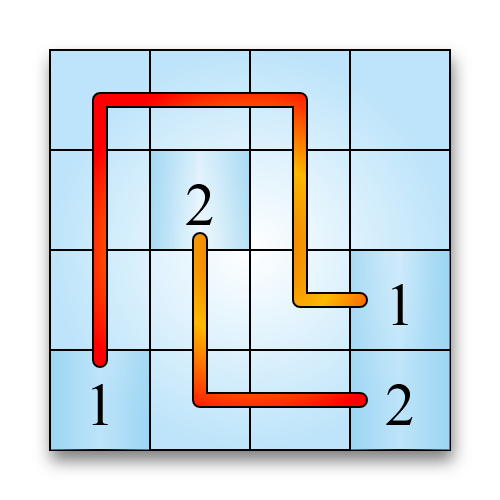
\includegraphics[width=0.4\textwidth]{images/example_4_1.png}
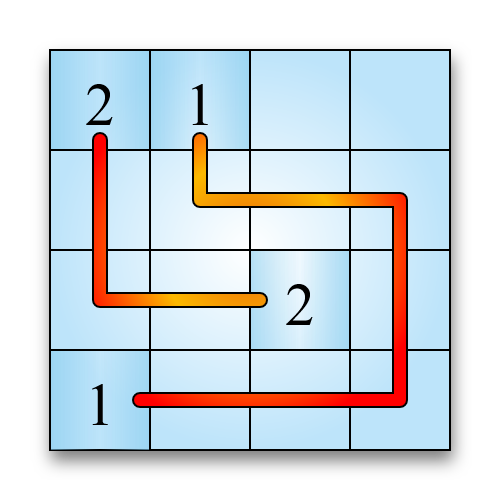
\includegraphics[width=0.4\textwidth]{images/example_4_2.png}
\subsection{Bsp. für $n=7$}
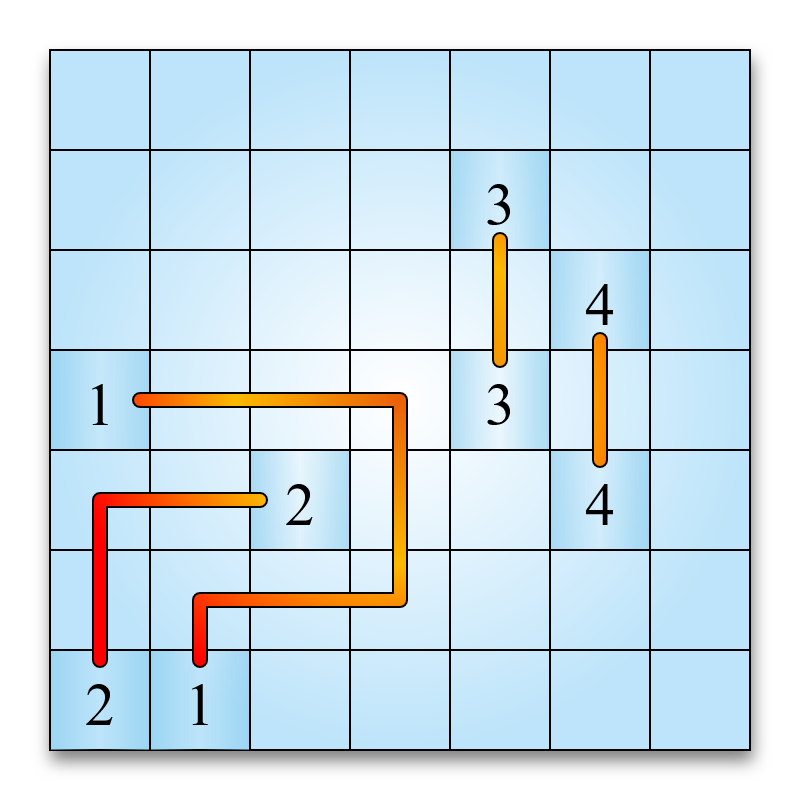
\includegraphics[width=0.4\textwidth]{images/example_7_1.png}
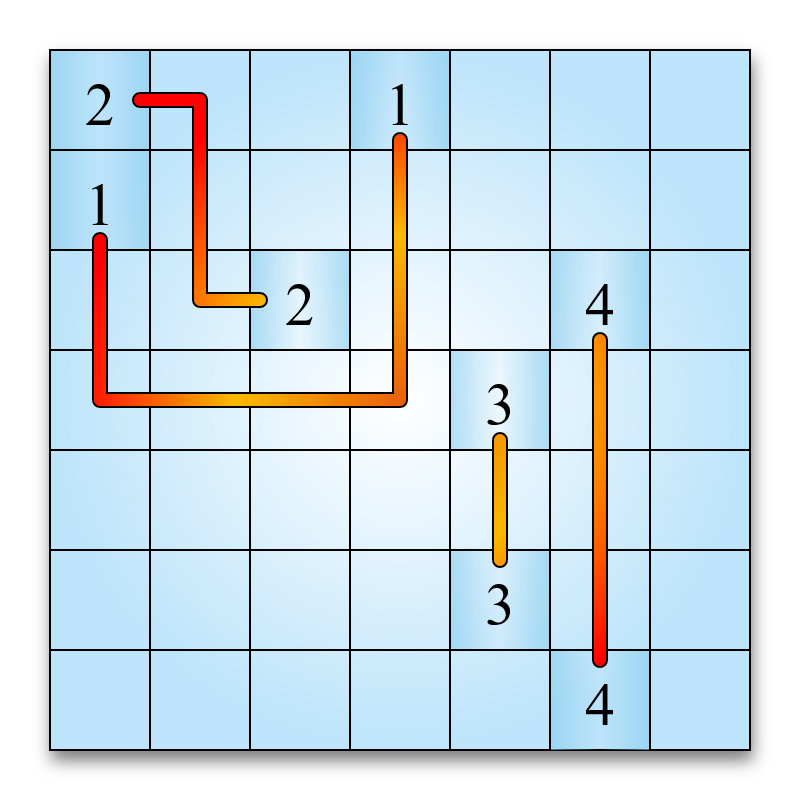
\includegraphics[width=0.4\textwidth]{images/example_7_2.png}
\subsection{Bsp. für $n=12$}
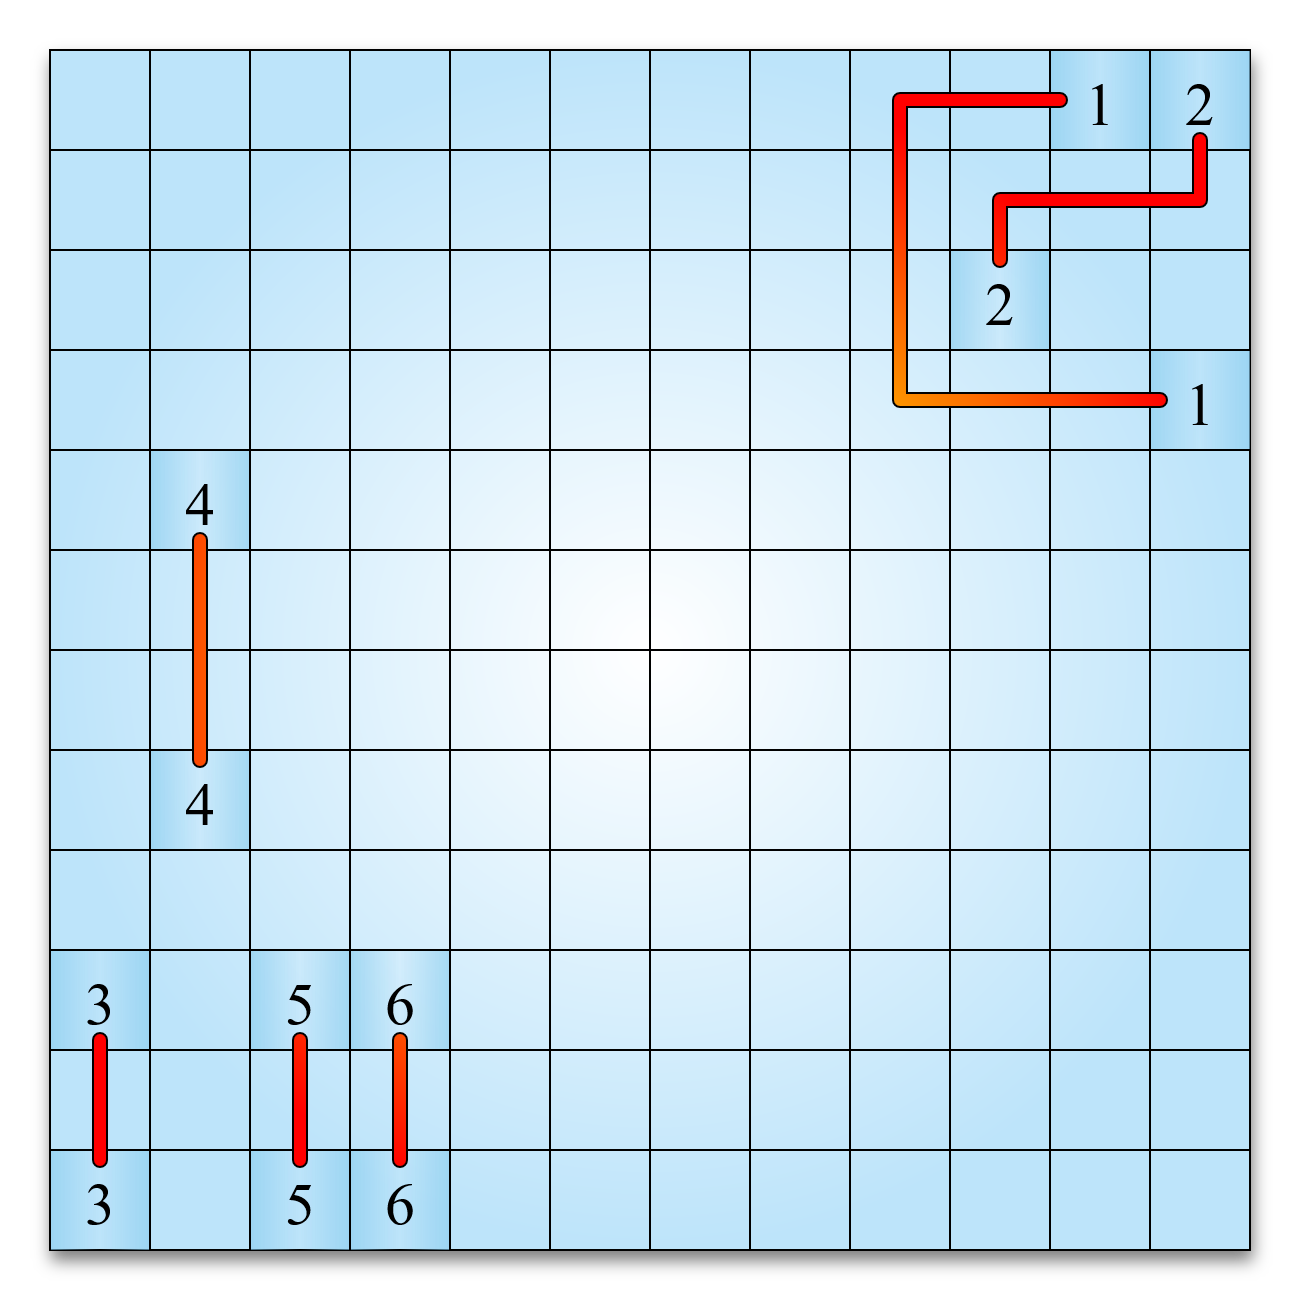
\includegraphics[width=0.6\textwidth]{images/example_12.png}
\subsection{Bsp. für $n=20$}
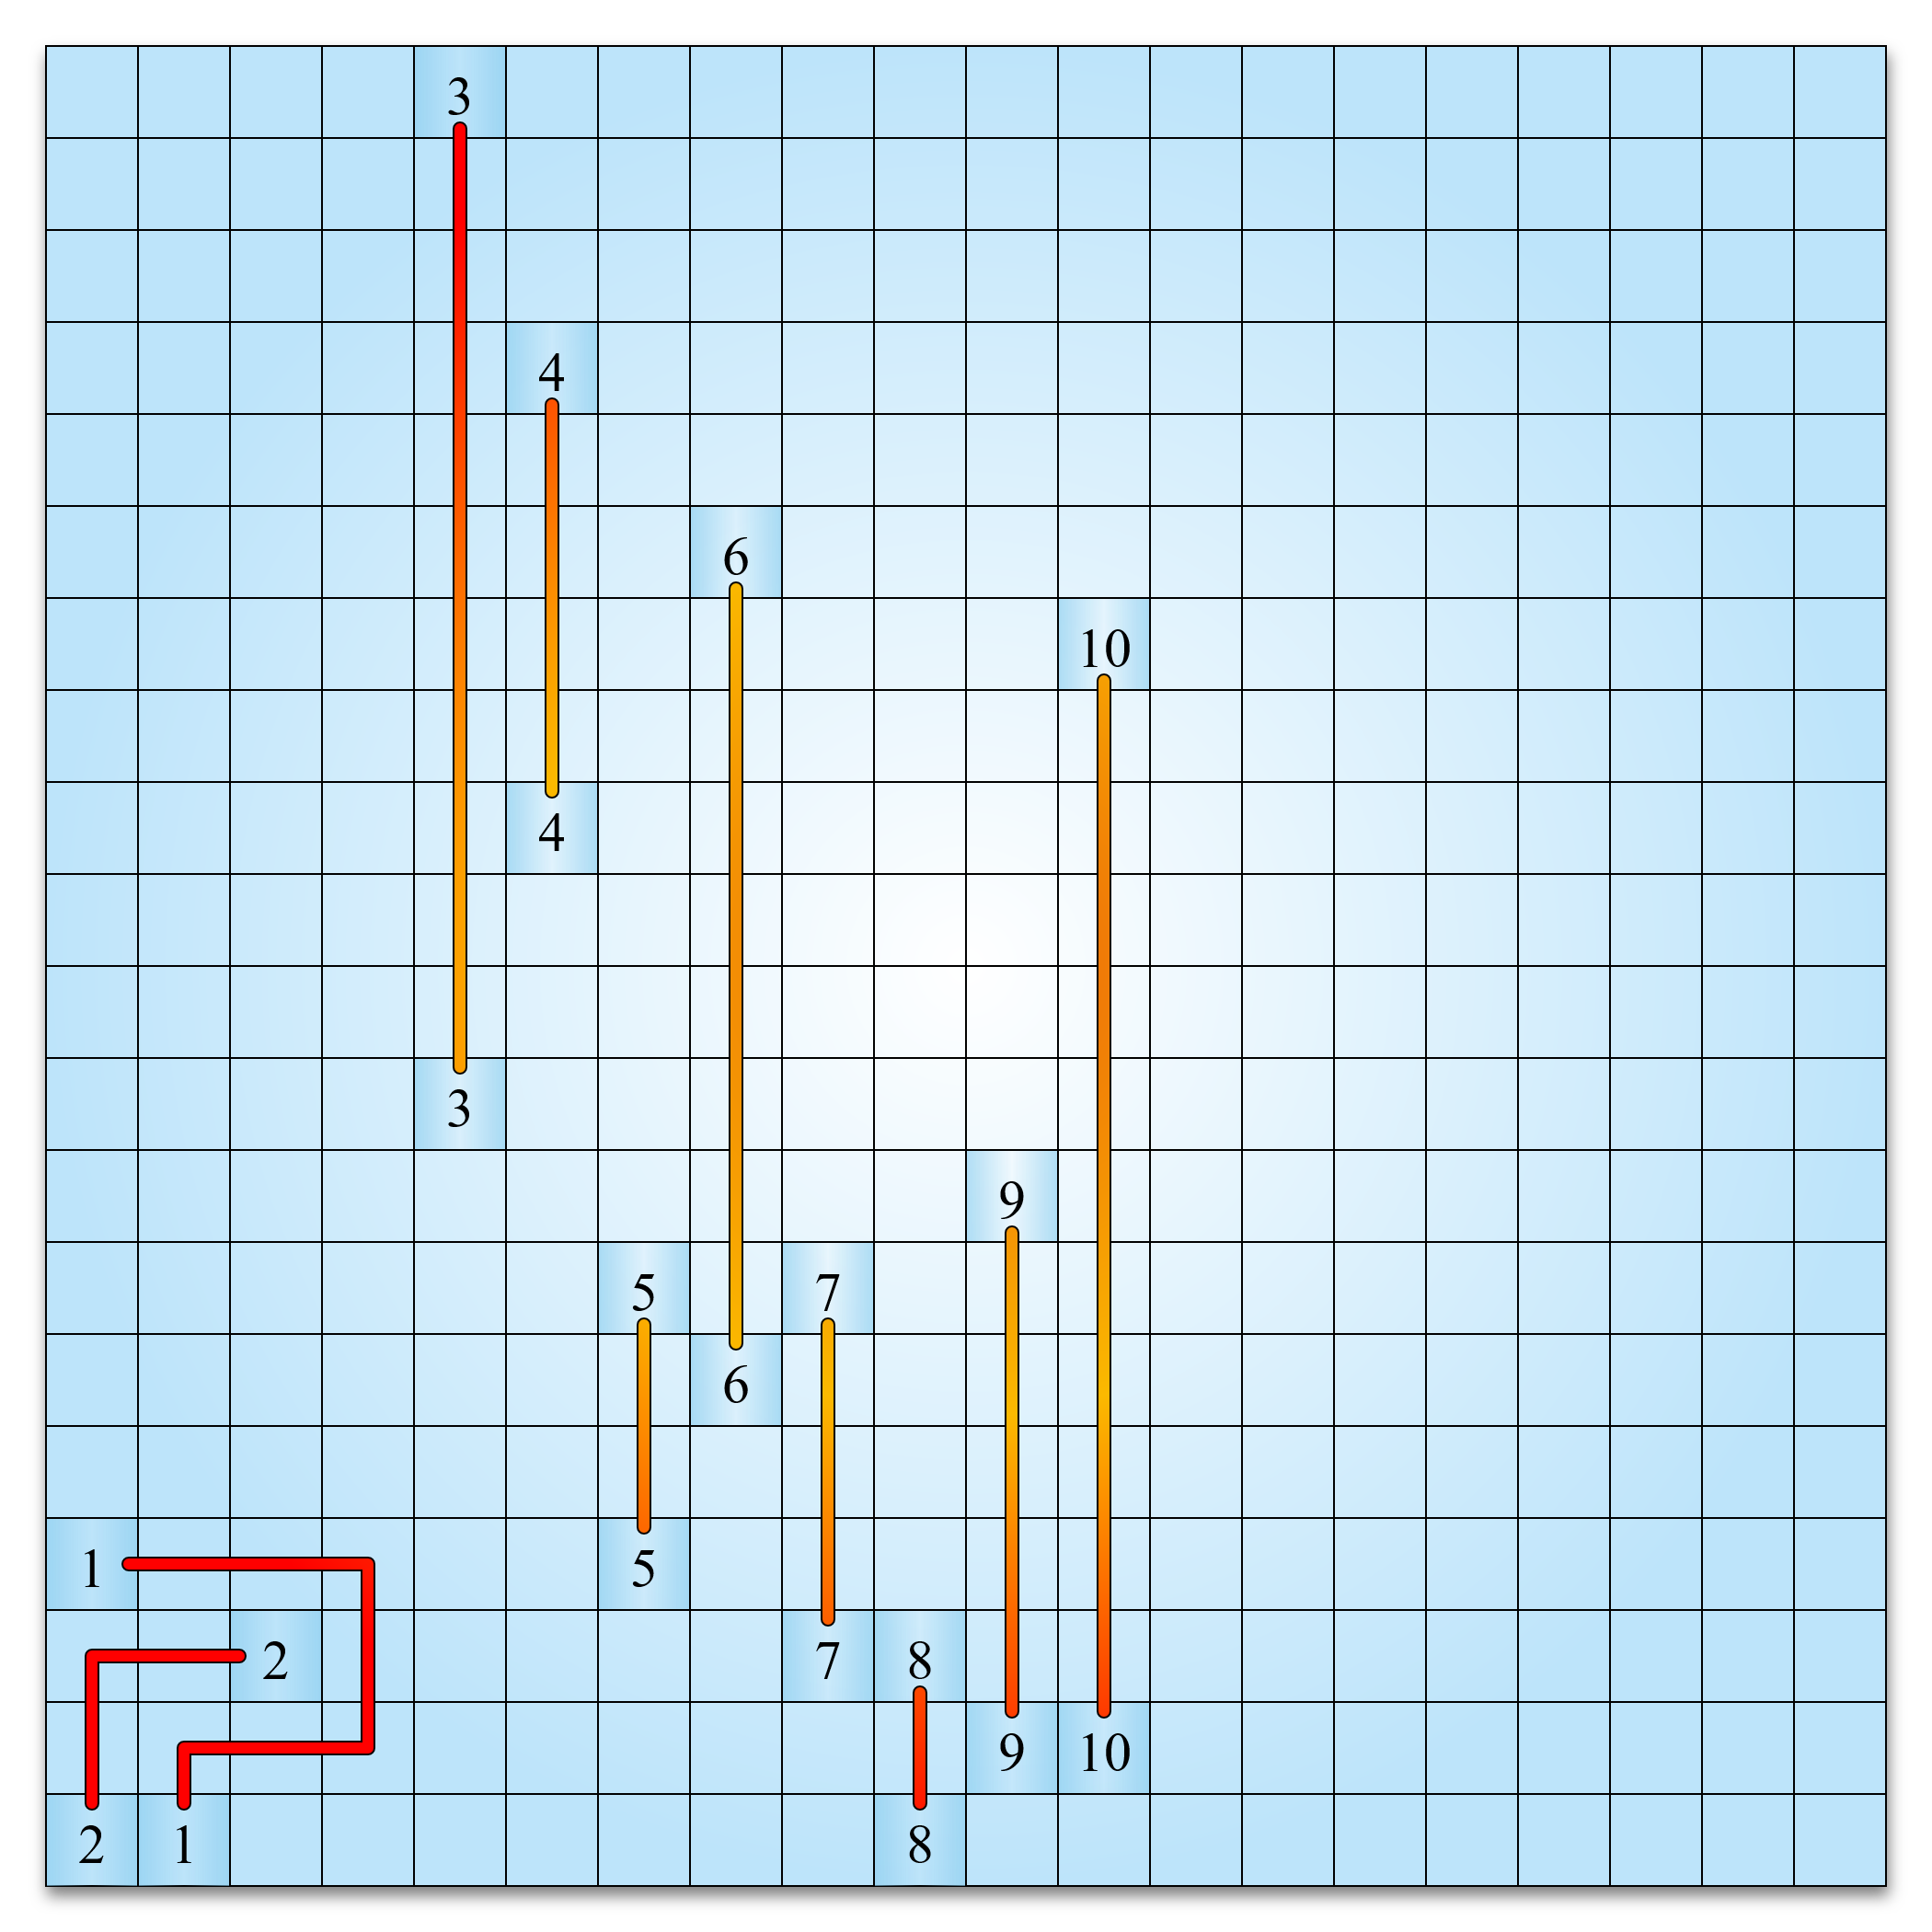
\includegraphics[width=0.8\textwidth]{images/example_20.png}
\subsection{Bsp. für $n=30$}
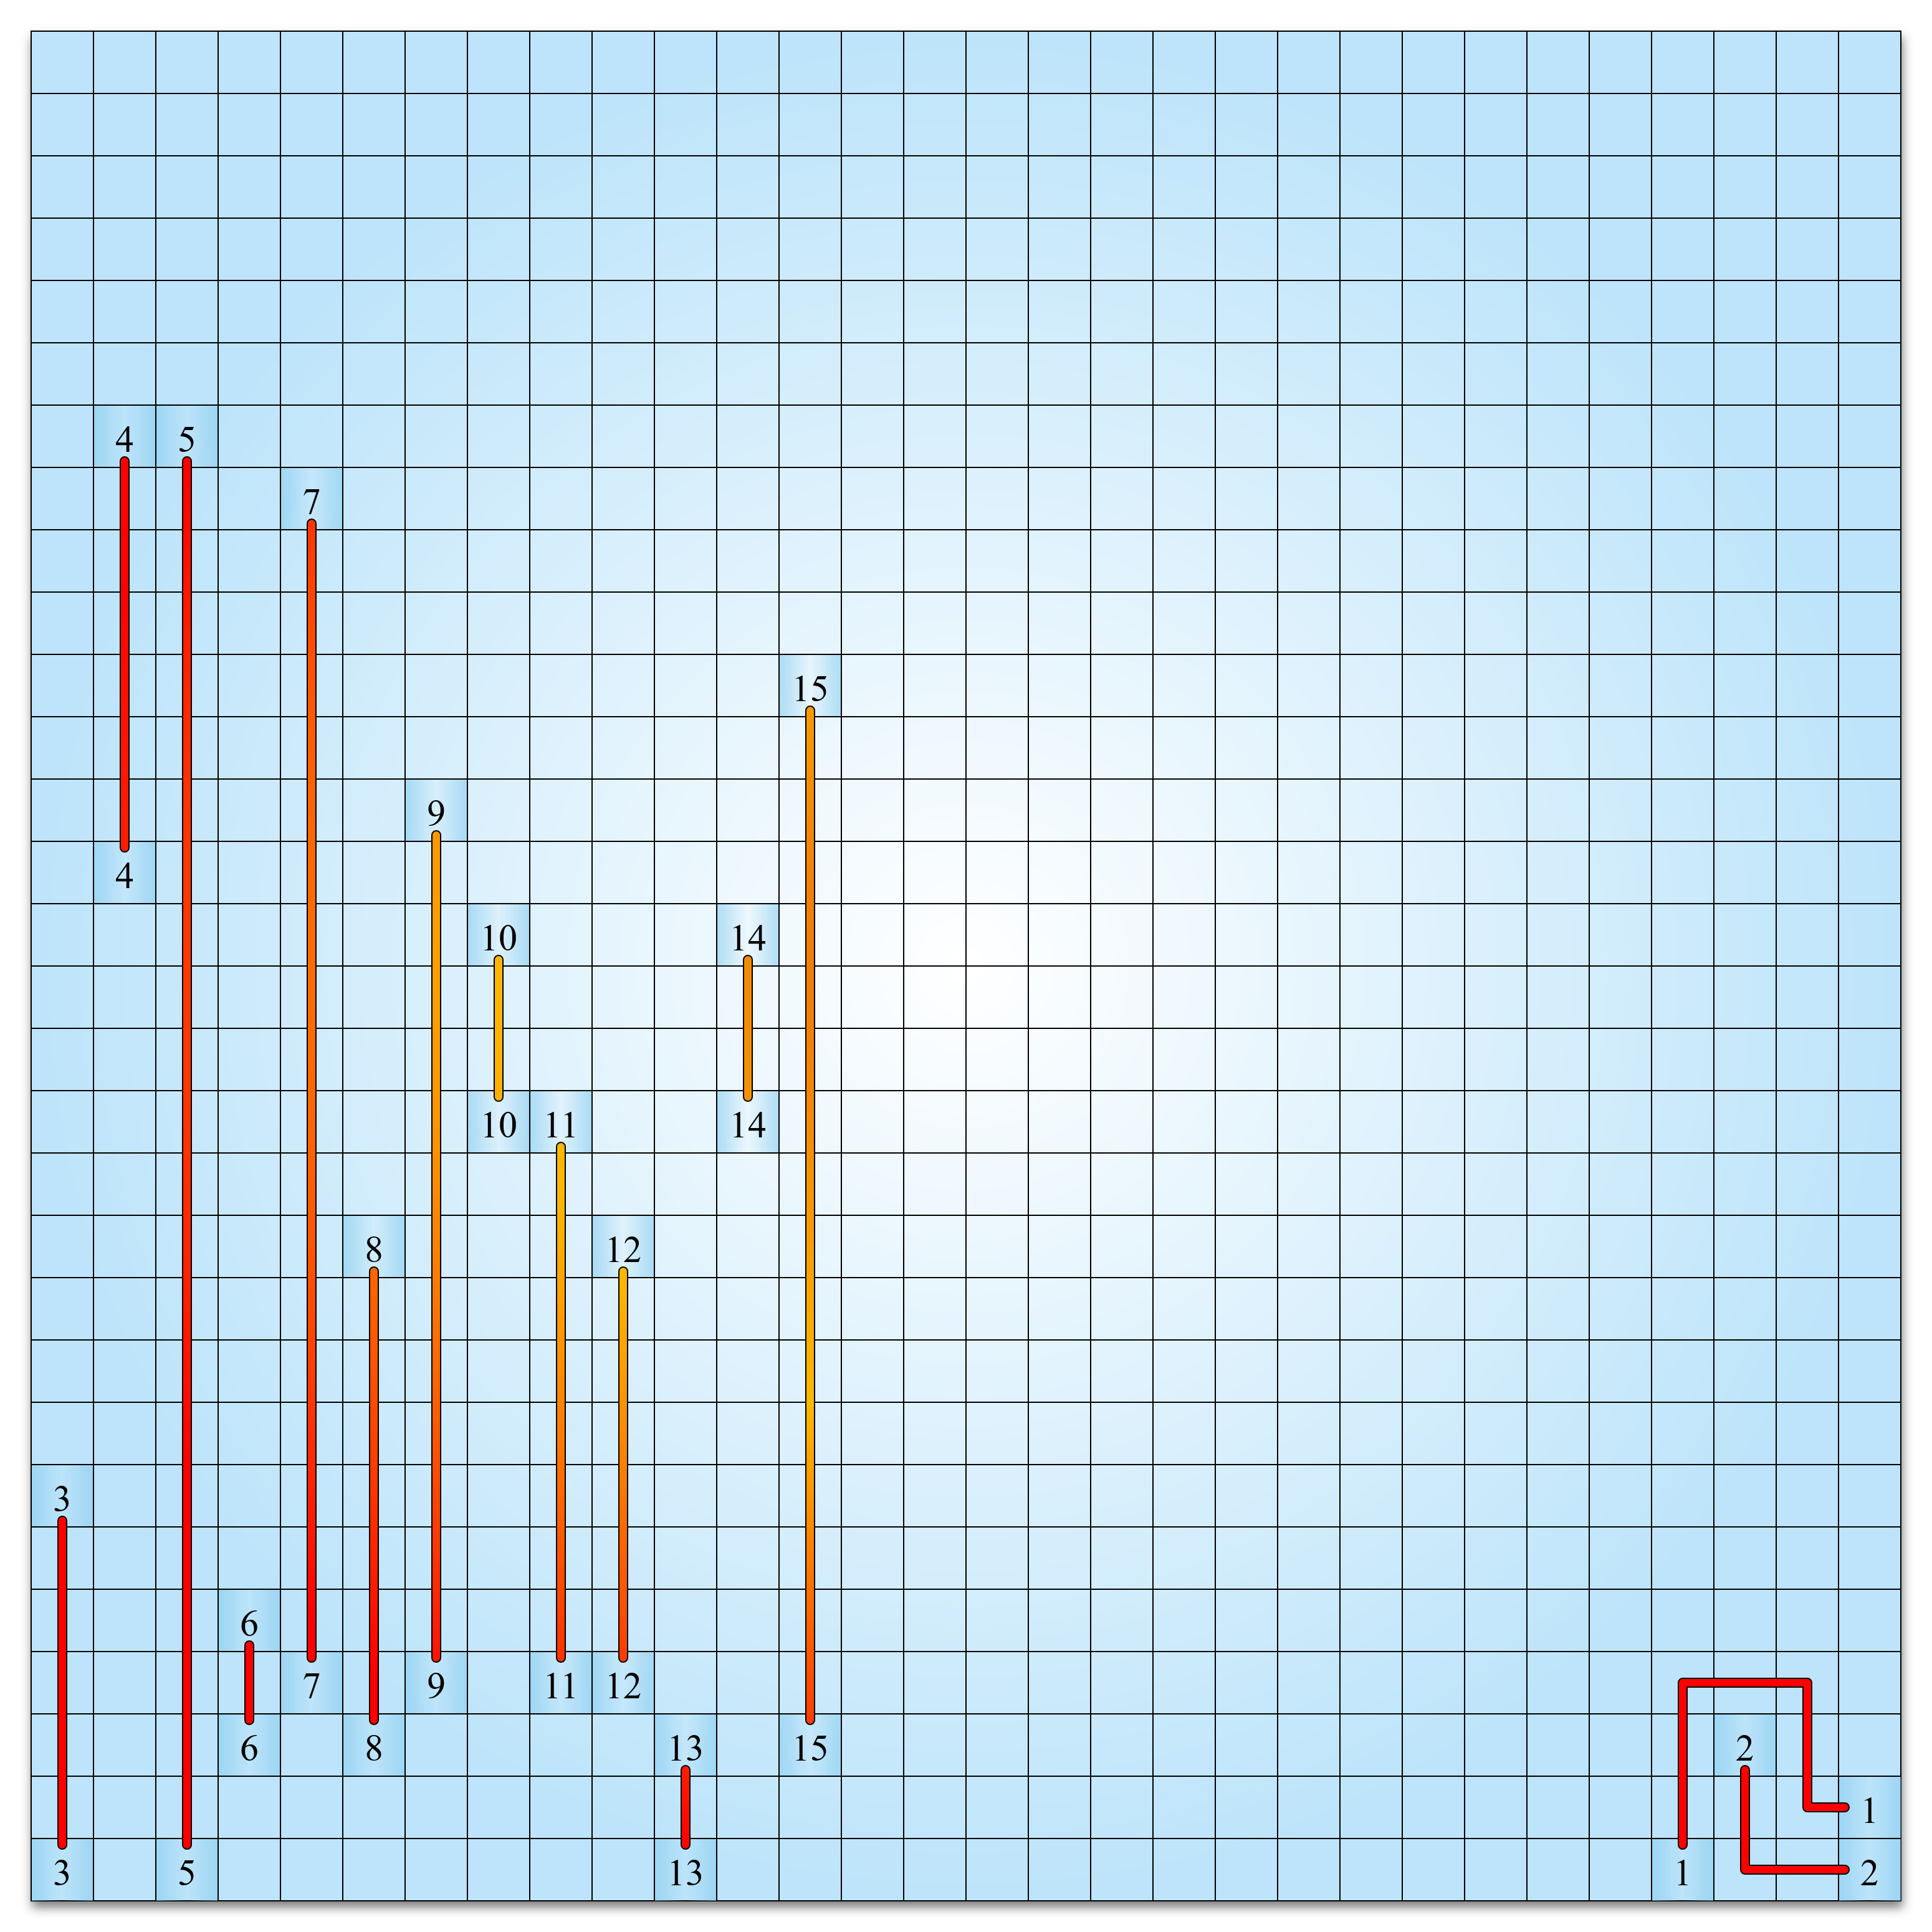
\includegraphics[width=\textwidth]{images/example_30.png}

\section{Quellcode}
\lstinputlisting[language=Python,title=arukone.py]{../arukone.py}


\end{document}
